%====================================================
%
% Author: DR. XAVIER NOUMBISSI NOUNDOU
%
%====================================================
\documentclass[12pt, a4paper]{article}
\NeedsTeXFormat{LaTeX2e}

%---------------------------- PACKAGE INCLUSION -------------------------------
% This group renders characters clearer and more precise

\RequirePackage[bitstream-charter,cal,expert]{mathdesign}
\RequirePackage{latexsym}

\usepackage{geometry}
\geometry{a4paper,
		  %showframe=true,
		  %margin=2.75em,
		  %a4paper,
		  %total={170mm,257mm},
		  top=3.5em,
		  left=3em,
		  right=3em,
		  bottom=3.39em
		  }

\usepackage[default]{cantarell}
\usepackage{graphicx}
\usepackage{xspace}
\usepackage[parfill]{parskip} % Activate to begin paragraphs with an empty line rather than an indent
\usepackage{paralist} % very flexible & customisable lists (eg. enumerate/itemize, etc.)
\usepackage{listings} % for lstset definitions
\usepackage{url}
\usepackage{subfig} % make it possible to include more than one captioned figure/table in a single float
\usepackage{epsfig}
\usepackage{booktabs}
%\usepackage{enumitem} %funny itemize icons
\usepackage{verbatim}
\usepackage{tcolorbox}

\usepackage{pagecolor}

\usepackage{amsmath}
\newcommand{\mathbold}[1]{\text{\textbf{#1}}}

\usepackage{xcolor}
\definecolor{yerothColorOrange}{RGB}{242, 161, 0}   
\definecolor{yerothColorBlue}{RGB}{77 , 93 , 254}
\definecolor{yerothColorRed}{RGB}{254, 48 , 48}
\definecolor{yerothColorGray}{RGB}{198, 198, 198}
\definecolor{yerothColorDarkgray}{RGB}{60, 60 , 60}
\definecolor{yerothColorIndigo}{RGB}{83, 0, 125}
\definecolor{yerothColorGreen}{RGB}{2  , 160, 70}
\definecolor{forestgreen}{RGB}{2,160,70}    
\definecolor{mediumblue}{RGB}{7,43,205}    
\definecolor{firebrickred}{RGB}{178,34,34}
\definecolor{listingray}{gray}{0.9}
\definecolor{lbcolor}{rgb}{0.9,0.9,0.9}
\definecolor{darkgreen}{rgb}{0,0.35,0}
\definecolor{medgreen}{rgb}{0,0.5,0}
\definecolor{lightgreen}{rgb}{0.5,0.7,0.5}
\definecolor{pmcolour}{rgb}{0.5,0.7,0.5}
\definecolor{medgrey}{rgb}{0.6,0.6,0.6}
\definecolor{purplish}{rgb}{0.4,0,0.6}
\definecolor{brightred}{rgb}{1,0.2,0.2}

\newcommand{\diplinfn}{DR.\xspace}

\newcommand{\yerothrc}{\textcolor{yerothColorGreen}
			{\textsc{\textcolor{yerothColorRed}{YEROTH}}$_{\text{r\&c}}$\xspace}}

\newcommand{\yerotherpblack}{YEROTH--ERP--$3.0$\xspace}

\newcommand{\erpcustombuiltIESAPone}{Custom--built (i.e.: SAP Business One)\xspace}

\newcommand{\erpcustombuiltIESAP}{Custom--built (i.e.: SAP)\xspace}

\newcommand{\yerotherp}{\textsc{\textcolor{yerothColorBlue}{YEROTH--ERP--$3.0$}}\xspace}

\newcommand{\sageerp}{Sage Gescom i$7$\xspace}

\newcommand{\myfullacademicname}{DR. XAVIER NOUMBISSI NOUNDOU\xspace}

\usepackage{hyperref}
\hypersetup{
    colorlinks,
	pagebackref,
    citecolor=medgreen,
    linkcolor=purplish,
    breaklinks,
    pdftex,
    bookmarks,
    plainpages=false,
	pdftitle={Advantages of \yerotherpblack compared to top tier--1 ERP
			  software--systems. Authored by: ''\myfullacademicname''.},
    pdfauthor={\myfullacademicname}
}

%--------------------------------------------------------------------------------

%---------------------------- COMMANDS DEFINITION -------------------------------
\newcommand{\diplinf}{\emph{Dipl.-Inf.}\xspace}
\newcommand{\mycheckmark}[1]{\textcolor{#1}{$\checkmark$}\xspace}

\newcommand{\myenumitem}[1]{\emph{#1}\xspace}
\newcommand{\yerenalert}{\emph{yeren-alert}\xspace}

\newcommand{\erpsoftware}{ERP~software--system\xspace}

\newcommand{\mysql}{MySQL\xspace}
\newcommand{\mysqlcolored}{\textcolor{yerothColorBlue}{My}\textcolor{yerothColorOrange}{SQL}\xspace}

\newcommand{\yerothvert}[1]{\textcolor{yerothColorGreen}{#1}\xspace}
\newcommand{\yerothorange}[1]{\textcolor{yerothColorOrange}{#1}\xspace}
\newcommand{\yerothrouge}[1]{\textcolor{yerothColorRed}{#1}\xspace}

\newcommand{\yerothfacile}{\yerothvert{easy}\xspace}
\newcommand{\yerothdifficile}{\yerothorange{difficult}\xspace}
\newcommand{\yerothtresdifficile}{\yerothrouge{very difficult}\xspace}

\newcommand{\featuresummary}[2]{\textbf{\textcolor{#1}{\textsc{#2}}}}

%--------------------------------------------------------------------------------

\usepackage[T1]{fontenc}
\newcommand{\changefont}[3]{
\fontfamily{#1} \fontseries{#2} \fontshape{#3} \selectfont}
\changefont{cmss}{m}{n}

\renewcommand\labelenumi{\theenumi)}

\pagenumbering{gobble}

\usepackage{fancyhdr}
\pagestyle{fancy}
\renewcommand{\headrulewidth}{0pt}
\rhead{}
\lhead{}
\lfoot{{\small Author: \myfullacademicname}}
\rfoot{{\small Version of --~\today~--}}
\cfoot{}

\clubpenalty = 10000
\widowpenalty = 10000
\displaywidowpenalty = 10000

\begin{document}

{\bf \Large \yerothrc} {| \sc \scriptsize advantages of \yerotherpblack compared
				to top tier--1 ERP software--systems}

\vspace{2.5em}

\parbox{27em}{\LARGE Advantages of \yerotherpblack Compared
				to Top Tier--1 ERP Software--Systems}

\vspace{0.5em}

\begin{table}[!htbp]
\begin{tabular}{ll}
\parbox{27em}{
\yerotherpblack is a very easy to use ERP (Enterprise Resource Planing)
software--system because of its characteristics:
\vspace{0.5em}
\begin{enumerate}[1.]
	\itemsep 0.2em
	\item separate views for each user role
	\item complete and fundamental training in $5$ days
	\item easy to use graphical user interface (GUI)
	\item no college or university training needed
	\item no formal business training needed
	\item no financial accounting training needed
	\item no internet connection needed.\\
\end{enumerate}
}

&

\parbox{15em}{
\begin{center}
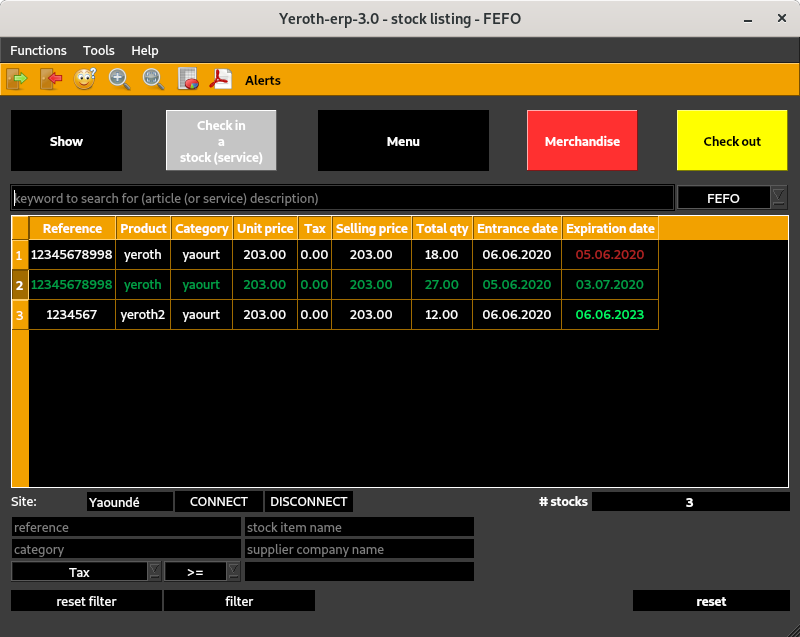
\includegraphics[scale=0.25]{images/yeroth-stock-listing-window.png}
\caption*{Stock listing window}
\end{center}
}
\end{tabular}
\end{table}

\vspace{0em}

Table~\ref{tab:comparison-against-others-erp-software-systems}
pictures the 'effectiveness' and 'simplicity' of \yerotherpblack, 
compared to top tier--1 ERP software--systems ''\sageerp'',
and ''\erpcustombuiltIESAPone''.\\

\vspace{-1.2em}

\begin{table}[!htbp]
\centering
\begin{tabular}{cccc} 

\multicolumn{1}{c}{}			&
\yerotherpblack 				& 
\sageerp						&
\erpcustombuiltIESAP 			\\ \hline

separate views per user role	&
		\yerothvert{YES}		&
		\yerothrouge{NO}		&
		\yerothvert{YES}		\\ \hline

reusable for multiple purposes	&
		\yerothvert{yes}		&
		\yerothvert{yes}		&	
		\yerothrouge{no*}		\\ \hline

complete training					&
		\yerothvert{$5$ days}		&
		\yerothorange{$2$ months}	&	
		\yerothrouge{$3$ months}	\\ \hline

difficulty in navigation			&
		\yerothfacile				&
		\yerothdifficile			&
		\yerothtresdifficile		\\  \hline
		
usage language in software					&
		\yerothvert{easy everyday English}	&
		\yerothorange{simple}				&
		\yerothrouge{technical}				\\ \hline			
		
financial accounting knowledge	&
		\yerothvert{no}			&
		\yerothvert{no}			&
		\yerothorange{useful}	\\ \hline		

advanced marketing knowledge	&
		\yerothvert{no}			&
		\yerothorange{useful}	&
		\yerothorange{useful}	\\ \hline
		
internet connection				&
		\yerothvert{optional}	&
		\yerothrouge{mandatory}	&
		\yerothvert{optional}	\\ 
\end{tabular}
\caption{Comparison between \yerotherpblack and $2$ top tier--1
	full featured ERP software--systems\\}
\label{tab:comparison-against-others-erp-software-systems}
\end{table}

\vspace{-1.6em}

{\large \bf OPERATIONS}

\vspace{-0.6em}

\begin{table}[!htbp]
\begin{tabular}{lll}

\begin{tcolorbox}[width=14.3em, boxrule=0.01em, colback=white]
\textbf{Point--of--Sale Hardware}
\vspace{-1em}
\hrule
\vspace{0.75em}
\begin{itemize}[]
	\item[\mycheckmark{yerothColorDarkgray}] Barcode scanner
	\item[\mycheckmark{yerothColorDarkgray}] Thermal printer, etc.\\
\end{itemize}
\begin{center}
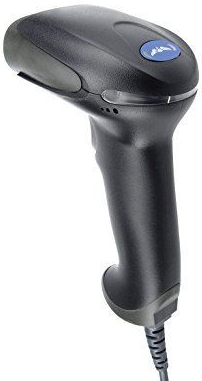
\includegraphics[scale=0.24]{images/xfox-fj-5-usb-plug-and-play-automatic-barcode-scanner.png}
\end{center}
\end{tcolorbox}

&

\begin{tcolorbox}[width=14.3em, boxrule=0.01em, colback=white]
\textbf{Database Management Systems}
\vspace{0.1em}
\hrule
\vspace{0.75em}
\begin{itemize}[]
	\item[\mycheckmark{yerothColorBlue}] \mysqlcolored\\
\end{itemize}
\begin{center}

\includegraphics[scale=0.14]{images/free-reuse-dbms-logo}
\end{center}
\end{tcolorbox}

&

\begin{tcolorbox}[width=14.3em, boxrule=0.01em, colback=white]
\textbf{Operating Systems}
\vspace{0.1em}
\hrule
\vspace{0.75em}
\begin{itemize}[]
	\item[\mycheckmark{yerothColorRed}] Debian--Linux\\	
\end{itemize}
\begin{center}

\includegraphics[scale=0.53]{images/free-reuse-stretch-logo}
\end{center}
\end{tcolorbox}

\end{tabular}
\end{table}


\end{document}

